\documentclass[../main.tex]{subfiles}
\graphicspath{{\subfix{../images/}}}
\begin{document}
Assume $(X,Y)$ distributes with joint density function
$f(x,y\mid\theta)=e^{-(x\theta+\frac{1}{\theta} y)}$.
(Slight correction: the function as it appears here is not strictly a  distribution, that is because the integral over all of the plane is infinite. after talking to the T.A. it was corrected to
$f'(x,y):= e^{-(x\theta+\frac{1}{\theta}y)}\cdot \mathbbm{1}_{\{x,y>0\}})$
\begin{enumerate}

    \item Show that the Fischer information on n samples is 
    $I(\theta)=\frac{2n}{\theta^2}$

    \item Show that $(T,U)$ is a sufficient statistic, yet is not complete where    
    \[T:=\sqrt{\sum_i Y_i\big/\sum_i X_i},\text{ and } U:=\sqrt{\sum_i Y_i\sum_i X_i}\]
    
    \item Show that T is an MLE for $\theta$
    
    \item Is T a UMVUE? Can we know whether there is a UMVUE using Lehman-Scheffe?
    
    \item Calculate the first 2 moments $\mathbb{E}[T],\mathbb{E}[T^2]$ (Hint: Use the gamma function)

    \item Define
    \[z_1:=(n-1)\big/\sum_i X_i,\text{ and } z_2:=\sum_i Y_i\big/n\]
    Show that they are unbiased estimators for $\theta$, and calculate their variance. 
    
    \item Find the best estimator of the form
    $\alpha z_1+(1-\alpha) z_2$
    What is it's variance? Compare to T's variance after the removal of the bias. 
\end{enumerate}
\noindent\line(1,0){480}
\subsection*{Solution:}
The first thing we will do is notice that we can decompose the distribution in the following way
\[f(x,y) = \left(\theta\cdot e^{-x\theta}\cdot\mathbbm{1}_{\{x>0\}}\right)\cdot \left(\frac{1}{\theta}\cdot e^{-y/\theta}\cdot\mathbbm{1}_{\{y>0\}}\right)\]
And so notice that if we take $Z_1\sim\text{Exp}(\theta),Z_2\sim\text{Exp}(\frac{1}{\theta})$ independently distributed random variables, we have that the joint density function of $(Z_1,Z_2)$ is exactly that of our original $(X,Y)$. This means that 
\[(X,Y)\overset{d}{\equiv}(Z_1,Z_2)\]
That means we can think of X as an $\text{Exp}(\theta)$ random variable and that it is independent of Y which is an $\text{Exp}(\frac{1}{\theta})$ random variable. We will use this throughout the solution. Now we will return to the solution of the problem. 

\begin{enumerate}
    
    \item Remember that under enough regularity assumptions we have that the Fischer-information is
    \[I(\theta) = -\mathbb{E}\left[\frac{d^2}{d\theta^2} \log\left(f_{\theta}(\overrightarrow{y})\right)\right]\]
    \emph{(The regularity assumptions are basic ones that a simple exponential function obviously satisfies, like the twice differentiability criteria or being able to change order between differentiation and integration and the support being independent of $\theta$.)}
    First we will find $f_{\theta}(\overrightarrow{y})$. 
    \begin{align*}
        f_{\theta}(\overrightarrow{y})&=\prod_{i=1}^n e^{-(x_i\theta+ y_i/\theta)} = e^{-\theta\sum_{i=1}^n x_i - \frac{1}{\theta}\sum_{i=1}^n y_i} \\
        \log f_{\theta}(\overrightarrow{y}) &= -\theta\sum_{i=1}^n x_i-\frac{1}{\theta}\sum_{i=1}^n y_i \\
        \frac{d}{d\theta}\log f_{\theta}(\overrightarrow{y}) &= -\sum_{i=1}^n x_i+\frac{1}{\theta^2} \sum_{i=1}^n y_i\\
        \frac{d^2}{d\theta^2}\log f_{\theta}(\overrightarrow{y}) &= -2\theta^{-3}\sum_{i=1}^n y_i
    \end{align*}
    And so
    \[\mathcolorbox{goodcolor}{I(\theta)} = -\mathbb{E}\left[\frac{d^2}{d\theta^2}\log f_{\theta}(\overrightarrow{y})\right] = \mathbb{E}\left[2\theta^{-3}\sum_{i=1}^n y_i\right]=2\theta^{-3}\mathbb{E}\left[\sum_{i=1}^n y_i\right] = 2\theta^{-3} \sum_{i=1}^n \mathbb{E}[y_i] = 2\theta^{-3}\cdot n\cdot\theta = \mathcolorbox{goodcolor}{\frac{2n}{\theta^2}}\]
    \[\left(\underline{\mathbb{E}[y_i]} = \int_0^\infty \frac{1}{\theta}\cdot t e^{-\frac{1}{\theta} t}dt = \frac{1}{\theta}\left(\left[-t\theta e^{-\frac{1}{\theta}y}\right]_{0}^{\infty} + \int_0^{\infty}\theta e^{-\frac{1}{\theta} t}dt\right) = \frac{1}{\theta}\cdot0 + \frac{1}{\theta} \left[-\theta^2 e^{-\frac{1}{\theta}t}\right]_0^{\infty} = \underline{\theta} \right)\]
    
    \qedsymbol
    
    \item First notice that $\frac{U}{T} = \sum_{i=1}^n X_i\text{, and } T\cdot U = \sum_{i=1}^n Y_i$. Now remember the Fisher-Neyman factorization theorem (see theorem \ref{Theorem: 1}), we will to try to factor the likelihood function -
    \[L(\theta; (\overrightarrow{x},\overrightarrow{y})):=\prod_{i=1}^n f_{\theta}(x_i,y_i) = \prod_{i=1}^n e^{-x_i\theta-\frac{1}{\theta} y_i} = e^{-\theta\sum_{i=1}^n x_i-\frac{1}{\theta}\sum_{i=1}^n y_i} = e^{-\theta\frac{U}{T} -\frac{1}{\theta} UT}\]
    Now we want to use the statistic $M= (U,T)$ for factorization. This means taking
    \begin{align*}g\left(M\left(\overrightarrow{X},\overrightarrow{Y}\right); \theta\right) &:= e^{-\theta\frac{U}{T} -\frac{1}{\theta} UT} \\ h\left(\overrightarrow{X},\overrightarrow{Y}\right)&:=1\end{align*}
    Now using the factorization theorem we have that \hlfancy{goodcolor}{$M=(T,U)$ is a sufficient statistic.} Now we also want to show that the statistic is not complete. Recall what a complete statistic is
    
    \begin{mdframed}[backgroundcolor=blue!20] 
        A statistic T is said to be complete if and only if for all measurable functions $g$:
        \[\forall\theta:\text{ } \mathbb{E}\left[g(T(\overrightarrow{Y}))\right]=0\Longrightarrow\forall\theta: \text{ }\mathbb{P}_\theta\left(g(T(\overrightarrow{Y}))=0\right)=1\]
    \end{mdframed}
    
    This implies that if we find a measurable function g on M such that
    \[\forall\theta:\text{ } \mathbb{E}\left[g(M(\overrightarrow{X}, \overrightarrow{Y}))\right]=0\text{ and  }\mathbb{P}_\theta\left(g(T(\overrightarrow{Y}))=0\right)\neq 1\]
    then we are done. Notice that
    \[\mathbb{E}\left[ U^2\right]= \mathbb{E}\left[\sum_i X_i\cdot \sum_i Y_i\right] = \sum_{i,j}\mathbb{E}[X_i\cdot Y_j] = n^2 \mathbb{E}[XY] = n^2\mathbb{E}[X]\mathbb{E}[Y] = n^2\theta\frac{1}{\theta} = n^2\]
    Where $\mathbb{E}[X]=\frac{1}{\theta}$, for the same reasons that $\mathbb{E}[Y] = \theta$. And so if we define $g(T,U)=U^2-n^2$, then we have
    \[\mathbb{E}\left[g\left(T,U\right)\right] = \mathbb{E}\left[U^2-n^2\right] = \mathbb{E}\left[U^2\right] - n^2 = n^2-n^2 = 0\]
    Notice that $U^2$ is not constant and so $g$ is not constant meaning we found a function $g$ that satisfies what we are looking for: \hlfancy{goodcolor}{$M=(T,U)$ is not a complete statistic.} \qedsymbol 
    
    \item Remember from the calculation of the fischer information that
    the log-likelihood is
    \[l\left(\theta;\left(\overrightarrow{x}, \overrightarrow{y}\right)\right) = -\theta\sum_{i=1}^n x_i-\frac{1}{\theta}\sum_{i=1}^n y_i\]
    Now we want to maximize this function (maximizing the likelihood is equivalent to maximizing the log-likelihood, since the log is monotone increasing), and so derive 
    \begin{align*}\frac{d}{d\theta} l(\theta;\left(\overrightarrow{x},\overrightarrow{y}\right)) &= -\sum_{i=1}^n x_i +\frac{1}{\theta^2}\sum_{i=1}^n y_i = 0 \Longrightarrow \theta^2\cdot \sum_{i=1}^n x_i = \sum_{i=1}^n y_i\Longrightarrow \\
    \Longrightarrow\theta^2 &= T^2 \Longrightarrow \underline{\theta = \pm T}
    \end{align*}
    Of course $T$ is positive and $\theta>0$ and so the only option is $\theta = T$. Now we will check whether or not this is a maximum. The second derivative is
    \[\frac{d^2}{d\theta^2} l(\theta;\left(\overrightarrow{x},\overrightarrow{y}\right)) = -\frac{2}{\theta^3}\sum_{i=1}^n y_i<0\]
    This is because $y_i>0,\theta>0$. And so if we take $\hat{\theta} = T$. We have a value of theta that maximizes the log-likelihood. And so \hlfancy{goodcolor}{$T$ is an MLE estimator for $\theta$.}\,\qedsymbol 
    
    \item Remember the following definition of a UMVUE - 
    
    \begin{mdframed}[backgroundcolor=blue!20] 
        \begin{definition} An estimator $\hat{\theta}$ is called an unbiased estimator with uniformly minimal variance (UMVUE) if it satisfies the following conditions
        \begin{enumerate}
            
            \item  $\hat{\theta}$ is an unbiased estimator.
            
            \item For any other unbiased estimator $\hat{\theta_1}$ 
        \[\text{Var}(\hat{\theta})\leq\text{Var}(\hat{\theta_1})\]
        For all $\theta\in\Theta$.
            
        \end{enumerate}
        \end{definition}
    \end{mdframed}
    
    If we determine that $T$ is a biased estimator for $\theta$ then we get that it is also not a UMVUE. This means showing that $\mathbb{E}[T]\neq \theta$. Notice that because $\{X_i\}\sim \text{Exp}(\theta)$ i.i.d. and $\{Y_i\}\sim \text{Exp}(\frac{1}{\theta})$ i.i.d. that we also have that
    \[R=\sum_{i=1}^n X_i\sim\Gamma \left(n, \frac{1}{\theta}\right), \text{ and }S=\sum_{i=1}^n Y_i \sim \Gamma\left(n, \theta\right)\Longrightarrow T=\sqrt{\frac{S}{R}}\]
    And so 
    \begin{align*}
        \mathbb{E}[T] = \mathbb{E}\left[\sqrt{\frac{S}{R}}\right] &= \int_0^\infty\int_0^\infty \sqrt{\frac{s}{r}} \cdot \frac{r^{n-1}\theta^n e^{-\theta r}}{\Gamma(n)}\cdot \frac{s^{n-1}e^{-\frac{1}{\theta} s}}{\Gamma(n)\theta^n}drds \\
        &=\frac{\Gamma(n-\frac{1}{2})\Gamma(n+\frac{1}{2})}{\Gamma(n)^2}\cdot \theta^{\frac{1}{2}}\cdot \theta^{\frac{1}{2}}\left(\int_0^\infty \frac{r^{n-\frac{1}{2}-1}\theta^{n-\frac{1}{2}}e^{-\frac{1}{\theta}r}}{\Gamma(n-\frac{1}{2})}dr\right)\cdot \left(\int_0^\infty \frac{s^{n+\frac{1}{2}-1} e^{-\theta s}}{\Gamma(n+\frac{1}{2})\theta^{n+\frac{1}{2}}}ds\right) \\
        &= \frac{\Gamma(n-\frac{1}{2})\Gamma(n+\frac{1}{2})}{\Gamma(n)^2}\cdot \theta \cdot \left(\int_0^\infty f_{\Gamma(n-\frac{1}{2}, \frac{1}{\theta})}(r)dr \right) \cdot \left(\int_0^\infty f_{\Gamma(n+\frac{1}{2}, \theta)}(s)ds \right)\\ &= \frac{\Gamma(n-\frac{1}{2})\Gamma(n+\frac{1}{2})}{\Gamma(n)^2}\cdot \theta
    \end{align*}
    Notice that this means that $\mathbb{E}[T]\neq \theta$, and so \hlfancy{goodcolor}{$T$ is biased and not a UMVUE}. \qedsymbol\\
    
    Recall the Lehmann-Scheffe theorem - 
    
    \begin{mdframed}[backgroundcolor=blue!20] 
        \begin{theorem}[Lehmann - Scheffe]
            If W is a sufficient and complete statistic for $\theta$, and T is an unbiased estimator then 
            \[T_1 = \mathbb{E}[T\mid W]\]
            Is a UMVUE for $\theta$. 
        \end{theorem}
    \end{mdframed}
    
    Meaning to invoke this theorem we need to have the existence of a sufficient and complete statistic. Remember from the lecture that a complete and sufficient statistic is also minimal, and so if we find a minimal sufficient statistic that isn't complete this means that there isn't a sufficient and complete statistic (These statistics should be functions of eachother which would mean that our non-complete minimal sufficient statistic should also be complete in contradiction). \\
    
    This means that if we can show that M is minimal then since it is not complete there aren't sufficient and complete statistics which would tell us we cannot use the Lehmann-Scheffe theorem. Remember from previous problems the criteria for minimality of a sufficient statistic - 
    \[\text{The ratio of the likelihoods of 2 samples is independent of }\theta\Longleftrightarrow\text{M agrees on the samples}\]
    Take 2 samplings $(\overrightarrow{x_1},\overrightarrow{y_1}), (\overrightarrow{x_2},\overrightarrow{y_2})$. Denote by $(T_1,U_1)$, $(T_2,U_2)$ the corresponding statistics. The ratio of the likelihoods is
    \begin{align*}\frac{L(\theta;(\overrightarrow{x_1},\overrightarrow{y_1}))}{L(\theta;(\overrightarrow{x_2},\overrightarrow{y_2}))} = \frac{e^{-\theta\frac{U_1}{T_1}}-\frac{1}{\theta}U_1T_1}{e^{-\theta\frac{U_2}{T_2}}-\frac{1}{\theta}U_2T_2} = e^{-\theta\left(\frac{U_1}{T_1}-\frac{U_2}{T_2}\right)-\frac{1}{\theta}\left(T_1U_1-T_2U_2\right)}\end{align*}
    For this to be independent of $\theta$ we need that 
    \[\left(\frac{U_1}{T_1}-\frac{U_2}{T_2}\right) = 0\text{, and }T_1U_1-T_2U_2 = 0\]
    And so we have that $T_1U_1 = T_2U_2\text{, and }T_1U_2=T_2U_1$. Notice that these are all positive and so we have that this is true if and only if $T_1=T_2\text{, and } U_1=U_2$. And so we have all together that 
    \[\text{The ratio of the likelihoods of 2 samples is independent of }\theta\Longleftrightarrow\text{ M agrees on the samples}\]
    Meaning we have proven that M is minimal sufficient yet not complete and for the reasons stated above we have that \hlfancy{goodcolor}{the theorem cannot be invoked in this case.} \qedsymbol
    
    \item Remember that we already calculated $\mathbb{E}[T]$ - 
        \[\mathcolorbox{goodcolor}{\mathbb{E}[T] = \frac{\Gamma(n-\frac{1}{2})\Gamma(n+\frac{1}{2})}{\Gamma(n)^2}\cdot \theta}\]
    So now what is left is to calculate $\mathbb{E}\left[T^2\right]$, we will do this in a very similar way - 
        \begin{align*}
        \mathcolorbox{goodcolor}{\mathbb{E}\left[T^2\right]} = \mathbb{E}\left[\frac{S}{R}\right] &= \int_0^{\infty}\int_0^{\infty} \frac{s}{r} \cdot\frac{r^{n-1}\theta^n e^{-\theta r}}{\Gamma(n)}\cdot \frac{s^{n-1}e^{-\frac{1}{\theta} s}}{\Gamma(n)\theta^n}dsdr \\
        &= \frac{\Gamma(n-1)\Gamma(n+1)}{\Gamma(n)^2}\cdot\theta\cdot\theta\cdot\left(\int_0^\infty \frac{r^{n-2}\theta^{n-1} e^{-\theta r}}{\Gamma(n-1)}dr\right)\cdot \left(\int_0^\infty \frac{s^{n}e^{-\frac{1}{\theta} s}}{\Gamma(n+1)\theta^{n+1}}ds\right) \\
        &= \frac{\Gamma(n-1)\cdot\left(n(n-1)\Gamma(n-1)\right)}{(n-1)^2\Gamma(n-1)^2}\cdot\theta^2\cdot \left(\int_0^\infty f_{\Gamma(n-1, \frac{1}{\theta})}(r)dr \right)\cdot \left(\int_0^\infty f_{\Gamma(n+1,\theta)}(s)ds \right) \\ &= \mathcolorbox{goodcolor}{\frac{n}{n-1}\theta^2}
    \end{align*}    
    \item We are supposed to show that $\mathbb{E}[z_1]=\mathbb{E}[z_2]=\theta$ - 
    \begin{align*}
        \mathcolorbox{goodcolor}{\mathbb{E}[z_1]}=\mathbb{E}\left[\frac{n-1}{R}\right]&=\int_0^{\infty} \frac{n-1}{r} \frac{r^{n-1}\theta^n e^{-\theta r}}{\Gamma(n)} dr = \frac{(n-1)\Gamma(n-1)}{\Gamma(n)}\int_0^\infty \frac{r^{n-2} \theta^{n-1} e^{-\theta r}}{\Gamma(n-1)} dr\\&=\frac{\Gamma(n)}{\Gamma(n)}\cdot\theta\cdot\left(\int_0^\infty f_{\Gamma(n-1,\frac{1}{\theta})}(r) dr\right) = \mathcolorbox{goodcolor}{\theta}\\
        \mathcolorbox{goodcolor}{\mathbb{E}[z_2]} = \mathbb{E}\left[\frac{S}{n}\right] &= \int_0^\infty \frac{s}{n}\cdot\frac{s^{n-1}e^{-\frac{1}{\theta} s}}{\Gamma(n)\theta^n}ds = \frac{\Gamma(n+1)}{n\Gamma(n)}\theta\cdot\int_0^{\infty} \frac{s^n e^{-\frac{1}{\theta}s}}{\Gamma(n+1)\theta^{n+1}} ds\\&=\frac{\Gamma(n+1)}{\Gamma(n+1)}\cdot\theta\cdot\left(\int_0^\infty f_{\Gamma(n+1,\theta)}(s) ds\right) =\mathcolorbox{goodcolor}{\theta}
    \end{align*}
    And so we have that they are unbiased estimators for $\theta$. The second moments are - 
    \begin{align*}
        \mathbb{E}\left[z_1^2\right] =\mathbb{E}\left[\frac{(n-1)^2}{R^2}\right] &= \int_0^\infty \frac{(n-1)^2}{r^2} \frac{r^{n-1}\theta^n e^{-\theta r}}{\Gamma(n)} dr = (n-1)^2\frac{\Gamma(n-2)}{\Gamma(n)}\theta^2\left(\int_0^\infty \frac{r^{n-3}\theta^{n-2}e^{-\theta r}}{\Gamma(n-2)}dr\right)\\ &= \frac{(n-1)^2}{(n-2)(n-1)}\theta^2\cdot \left(\int_0^{\infty}f_{\Gamma(n-2,\frac{1}{\theta})}(r)dr\right) = \frac{n-1}{n-2}\theta^2 \\
        \mathbb{E}\left[z_2^2\right] = \mathbb{E}\left[\frac{S^2}{n^2}\right] &= \int_0^{\infty}\frac{s^2}{n^2}\cdot\frac{s^{n-1}e^{-\frac{1}{\theta} s}}{\Gamma(n)\theta^n}ds = n^{-2}\frac{\Gamma(n+2)}{\Gamma(n)}\theta^2 \cdot\left(\int_0^{\infty}\frac{s^{n+1}e^{-\frac{1}{\theta}}s}{\Gamma(n+2)\theta^{n+2}} ds\right) \\ &=\frac{n(n+1)}{n^2}\theta^2\cdot \left(\int_0^{\infty}f_{\Gamma(n+2,\theta)}(s)ds\right) = \frac{n+1}{n}\theta^2
    \end{align*}
    And so the variances are
    \begin{align*}
        \mathcolorbox{goodcolor}{\text{Var}(z_1)} &= \mathbb{E}\left[z_1^2\right] - \mathbb{E}[z_1]^2 = \frac{n-1}{n-2}\theta^2 - \theta^2 = \mathcolorbox{goodcolor}{\frac{1}{n-2}\theta^2} \\
        \mathcolorbox{goodcolor}{\text{Var}(z_2)} &= \mathbb{E}\left[z_2^2\right] - \mathbb{E}[z_2]^2 = \frac{n+1}{n}\theta^2 - \theta^2 = \mathcolorbox{goodcolor}{\frac{1}{n}\theta^2}
    \end{align*}    
    \item Notice that $z_1$ and $z_2$ distribute independently and this is because $R$ and $S$ distribute independently. And so if we denote $z=z_1+z_2$. First notice that for every $\alpha$ this is an unbiased estimator for $\theta$, thus our objective would be to just minimize $\text{Var}(z)$.
    \[\text{Var}(z) = \text{Var}(\alpha z_1) + \text{Var}((1-\alpha)z_1) = \alpha^2\text{Var}(z_1)+(1-\alpha)^2\text{Var}(z_2) = \theta^2\left(\frac{\alpha^2}{n-2}+\frac{(1-\alpha)^2}{n}\right)\]
    We want to minimize this value, and so we will derive it according to $\alpha$ - 
    \[\frac{d}{d\alpha}\text{Var}(z) = \theta^2\left(\frac{2\alpha}{n-2} - \frac{2(1-\alpha)}{n}\right) = 0 \Longrightarrow \underline{\alpha=\frac{n-2}{2n-2}}\]
    And so since $\frac{d}{d\alpha}\text{Var}(z) = \theta^2\left(\frac{2}{n-2}+\frac{2}{n}\right)>0$, this means the above $\alpha$ minimizes the variance. And so the best estimator of this form and it's variance is 
    \[\mathcolorbox{goodcolor}{z=\frac{1}{2}\left(\frac{n-2}{\sum_i X_i} + \frac{\sum_i Y_i}{n-1}\right)\Longrightarrow \text{Var}(z) = \frac{(n-2)\theta^2}{(2n-2)^2}+\frac{n\theta^2}{(2n-2)^2} = \frac{\theta^2}{2n-2}}\]
    Remembering $\mathbb{E}[T]$, in order to remove the bias we need to define $\hat{T}:= \frac{\Gamma(n)^2}{\Gamma(n-\frac{1}{2})\Gamma(n+\frac{1}{2})}T$ to remove the bias. Now this means we want to compare the variance of $\hat{T}$ to the variance of the above z - 
    \begin{align*}
    \mathbb{E}\left[\hat{T}^2\right] &= \frac{\Gamma(n)^4}{\Gamma(n-\frac{1}{2})^2\Gamma(n+\frac{1}{2})^2}\mathbb{E}\left[T^2\right] = \frac{n\Gamma(n)^4\theta^2}{(n-1)\Gamma(n-\frac{1}{2})^2\Gamma(n+\frac{1}{2})^2} \Longrightarrow \\
    \Longrightarrow\text{Var}\left(\hat{T}\right) &= \mathbb{E}\left[\hat{T}^2\right] - \mathbb{E}\left[\hat{T}\right]^2 = \frac{\theta^2}{2(n-1)}\cdot 2 \left(\frac{n\Gamma(n)^4}{\Gamma(n-\frac{1}{2})^2\Gamma(n+\frac{1}{2})^2} - (n-1)\right)\\
    &= \text{Var}(z)\cdot 2 \left(\frac{n\Gamma(n)^4}{\Gamma(n-\frac{1}{2})^2\Gamma(n+\frac{1}{2})^2} - (n-1)\right)
    \end{align*}
    This is the plot of the coefficient function, this is done in the beginning of the code file submitted. There also is an explanation there for why this means \hlfancy{goodcolor}{$T$ is better than z as an estimate for $\theta$.} 
    
    \begin{mdframed}[backgroundcolor=blue!20]
        \begin{center}
            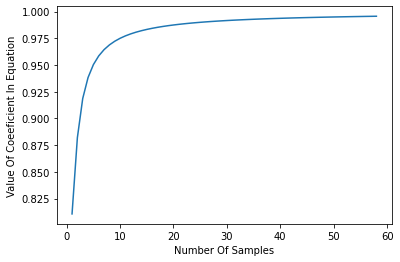
\includegraphics[scale=0.75]{images/WeirdFuncPlot.png}
        \end{center}
    \end{mdframed}

\end{enumerate}

\noindent\makebox[\linewidth]{\rule{\linewidth}{2pt}}


\end{document}